The inference part provides 4 functionalities:

\begin{itemize}
\item \mintinline{python}{romc.sample(n2, seed=None)}
\item \mintinline{python}{romc.eval_unnorm_posterior(theta)}
\item \mintinline{python}{romc.eval_posterior(theta)}
\item \mintinline{python}{romc.compute_expectation(h)}
\end{itemize}


\subsubsection*{\mintinline{python}{romc.sample(n2)}}

This is the basic inference utility of the ROMC implementation. The samples are drawn from a uniform distribution $q_i$ defined over the corresponding bounding box and the weight $w_i$ is computed as in equation~\eqref{eq:sampling}.


\subsubsection*{Example - Sampling}

\begin{minted}
[framesep=2mm,
baselinestretch=1.2,
fontsize=\small,
]
{python}
'''Sampling part'''
n2 = 20
tmp = romc.sample(n2=n2, seed=seed)

# visualize region, adding the samples now
romc.visualize_region(i=1)

# Visualise marginal (built-in ELFI tool)
romc.result.plot_marginals(weights=romc.result.weights, bins=100, density=True, range=(-3,3))
plt.show(block=False)

# Summarize the samples (built-in ELFI tool)
romc.result.summary()
### Prints ###
# Number of samples: 1720
# Sample means: theta: -0.0792

# compute expecation
print("Expected value   : %.3f" % romc.compute_expectation(h = lambda x: np.squeeze(x)))
# Expected value   : -0.079

print("Expected variance: %.3f" % romc.compute_expectation(h =lambda x: np.squeeze(x)**2))
# Expected variance: 1.061

\end{minted}

\begin{figure}[h]
    \begin{center}
      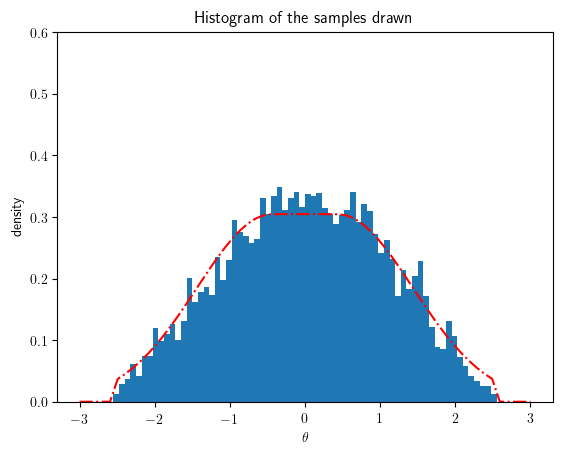
\includegraphics[width=0.48\textwidth]{./Thesis/images/chapter3/example_marginal.png}
      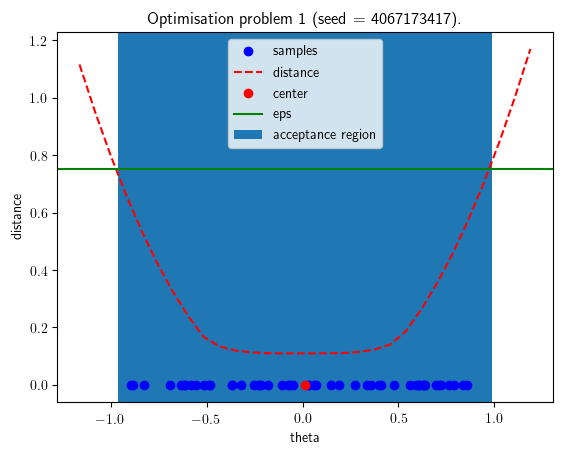
\includegraphics[width=0.48\textwidth]{./Thesis/images/chapter3/example_region_samples.png}
    \end{center}
  \caption{Histogram of distances and visualisation of a specific region.}
  \label{fig:example_training}
\end{figure}


\subsubsection*{Example - Evaluate Posterior}

The \pinline{romc.eval_unnorm_posterior(theta)} evaluates the posterior at point $\theta$ using the expression \eqref{eq:approx_posterior}. The \pinline{romc.eval_posterior(theta)} approximates the partition function $Z = \int_{\thetab} p_{d,\epsilon}(\thetab|\data) d\thetab$ using the Riemann approximation in the points where the prior has mass; hence it doesn't scale well to high-dimensional spaces. In our simple example, this utility can provide a nice plot of the approximate posterior.

\begin{minted}
[framesep=2mm,
baselinestretch=1.2,
fontsize=\small,
]
{python}
'''Evaluate posterior'''
tmp = romc.sample(n2=n2, seed=seed)

\end{minted}

\begin{figure}[h]
    \begin{center}
      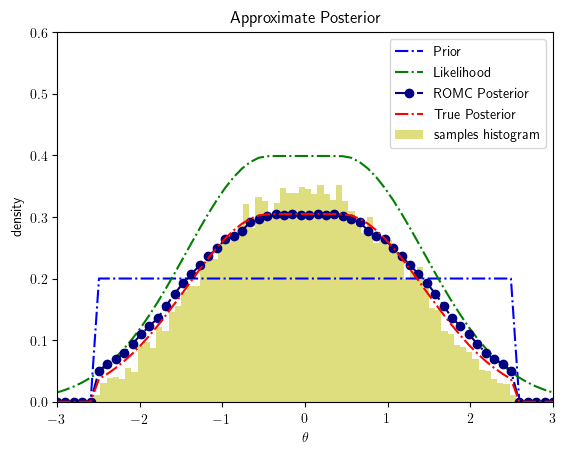
\includegraphics[width=0.75\textwidth]{./Thesis/images/chapter3/example_posterior.png}
    \end{center}
  \caption{Approximate posterior evaluation and histogram of the samples drawn.}
  \label{fig:example_posterior}
\end{figure}
